% Project-authored fixture: illustrative service-load measurements on a log axis.
\documentclass{article}
\usepackage{pgfplots}
\pgfplotsset{compat=1.18}

\title{Checkout API Load Test}
\author{Performance Engineering}
\date{September 2026}

\begin{document}
\maketitle

\section{Latency under concurrency}
This report compares median and 99th-percentile response times across five
concurrency levels. The measurements are illustrative. A logarithmic latency
axis keeps the rapid growth of the tail visible without hiding the median.

\begin{figure}
\centering
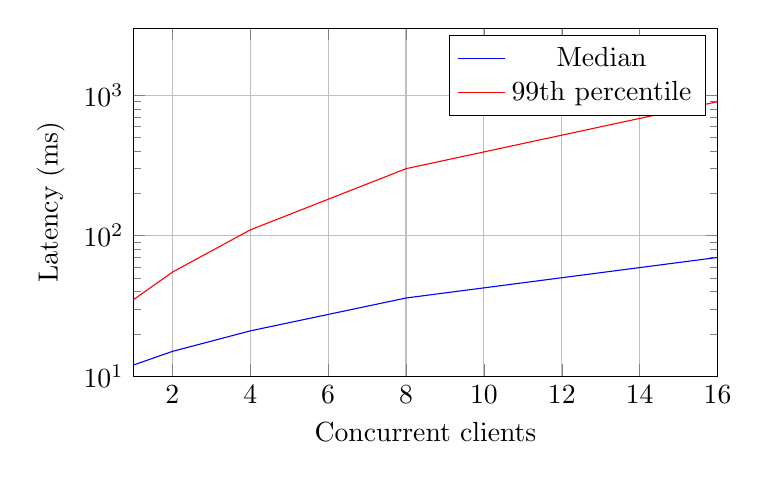
\begin{tikzpicture}
  \begin{semilogyaxis}[
    xmin=1,xmax=16,ymin=10,ymax=3000,
    width=9cm,height=6cm,
    xlabel={Concurrent clients},ylabel={Latency (ms)},grid=major]
    \addplot[blue] coordinates {
      (1,12) (2,15) (4,21) (8,36) (16,70)
    };
    \addlegendentry{Median}
    \addplot[red] coordinates {
      (1,35) (2,55) (4,110) (8,300) (16,900)
    };
    \addlegendentry{99th percentile}
  \end{semilogyaxis}
\end{tikzpicture}
\caption{Response-time distribution during a stepped load test.}
\label{fig:latency}
\end{figure}

The tail rises sharply after eight concurrent clients, while median latency
increases more gradually.
\end{document}
